%! Author = Len Washington III
%! Date = 9/29/2023

% Preamble
\documentclass[12pt]{report}

\usepackage[6]{cs430recitation}
\usepackage{algpseudocode}
\usepackage{cs430}

% Document
\begin{document}

%<*Recitation-6>
\subsection{After Lecture 09 \& 10 \& 11 \& 12} -- Answer any questions on HW3 (due today)\\
Practice Problems (all taken from previous exams)
\begin{enumerate}[label=\arabic*.]
	\item You should repeatedly use the $O(n)$ median algorithm to find the best choice for the order to insert values in a binary search tree to ensure that the binary search tree is balanced.
	\begin{enumerate}[label=\choicelabel]
	    \item True.
		\item \answer{False.}
	\end{enumerate}
	\item If you were just given the output of a traversal of a valid binary tree, could you draw the actual BST? Which of the following traversals is/are needed to draw the BST from given traversals.\begin{table}[H]
	    \centering
	    \begin{threeparttable}
			\label{tab:}
			\begin{tabular}{ccc}
				1) Inorder & 2) Preorder & 3) Postorder
			\end{tabular}
		\end{threeparttable}
	\end{table}
	\begin{enumerate}[label=\choicelabel]
	    \item Any one of the given three traversals is sufficient.
		\item \answer{Either 2 or 3 is sufficient.}
		\item Both 2 and 3 are needed.
		\item Both 1 and 3 are needed.
	\end{enumerate}
	\item The nodes of the following tree can be colored such that it is a red-black tree.
	\begin{figure}[H]
		\centering
		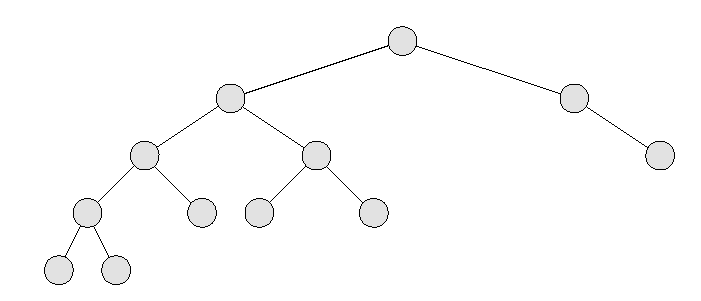
\includegraphics[width=\textwidth]{6.1}
		\label{fig:6.1}
	\end{figure}
	\begin{enumerate}[label=\choicelabel]
	    \item \answer{True.}
		\item False.
	\end{enumerate}
	\item Insert $20$, $15$, $5$, in that order, into an empty binary search tree. What rotations would be needed to balance the tree?
	\begin{enumerate}[label=\choicelabel]
	    \item Left rotation about node (5).
	    \item \answer{Right rotation about node (20).}
	    \item Left rotation about node (15), followed by a right rotation about node (20).
		\item No rotations are needed.
	\end{enumerate}
	\item Assume that you are given a ``black-box'' (i.e., you do not have the source code) procedure \Call{MEDIAN}{} that takes as parameters an array $A$ and subarray indices $p$ and $r$, and returns the value of the median element of $A[p\dots r]$ in $O(n)$ time in the worst case. Give a simple, recursive, linear-time algorithm that uses this procedure \Call{MEDIAN}{} to find the $i$th smallest element. Write the recurrence relation for your algorithm and show the solution is linear growth.\answer{
	\begin{algorithm}[H]
			\caption{}\label{alg:select}
			\begin{algorithmic}[1]
			\Function{Select}{A, p, r, i}
				\If{p == r}
					\State \Return A[p];
				\EndIf
			\EndFunction
			\end{algorithmic}
		\end{algorithm}
	}
	\item BST Given an arbitrary binary tree $T$ with integer keys stored at the nodes and pointers to the left and right sub binary trees, design an efficient algorithm which determines whether or not $T$ is a binary search tree. What is the time complexity of your algorithm?\answer{We may determine whether or not a given binary tree $T$ is a binary search}
	\item~\\
	\begin{enumerate}[label=\arabic{enumi}\alph*)]
	    \item Show each red-black tree that results after successively inserting the keys $4$ $7$ $12$ $15$ $3$ $5$ $14$ $18$ into an initially empty red-black tree. At the steps where a reb-black tree rule is violated, explain how it is corrected.
		\item Now delete these keys in this order and show each resultant red-black tree $18$ $15$ $7$ $14$. At the steps where a red-black tree rule is violated, explain how it is corrected.
	\end{enumerate}
	\item The external path length of a binary tree is the sum, taken over all nil leaves of the tree, of the depth of each leaf. Given the following binary search tree, in which internal nodes are shown as circles and external nodes (leaves; nil pointers) are shown as small boxes. The external path length (for nil leaves left to right) is $\mathbf{3 + 3 + 2 + 2 + 4 + 4 + 3 = 21 }$.
	\begin{enumerate}[label=\arabic{enumi}\alph*)]
	    \item 
		\begin{minipage}{0.5\textwidth}
			Is there a binary search tree on the same set of letters, $\{ D, G, N, Q, S, T \}$, that has lower external path length? Either give such a tree and how it is formed from the original BST or prove it does not exist. \answer{\sout{Yes, rotate the BST such that $Q$ is now the root.} Yes, we can reorganize the tree (rotate right at $T$, then rotate left at $Q$)}
		\end{minipage}
		\begin{minipage}{0.45\textwidth}
			\begin{figure}[H]
				\centering
				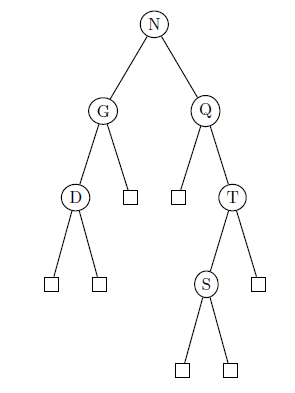
\includegraphics[width=\textwidth]{6.2}
				\label{fig:6.2}
			\end{figure}
			
		\end{minipage}
		\item Can the nodes in the original BST be colored red and black to form a proper red-black tree? \answer{Yes.} \correction{No, the root must be black. Then $G$ must be black (if it were red, $D$ would have to be black and blackheight from the root of the nil leaf at the right of $G$ would be 1, but the blackheight from the root to the nil leaves below $D$ would be 2) and $D$ must be red--this gives blackheight of 2 from the root to the nil leaves in the left subtree of $N$. In the right subtree of the root, the balckheight from $N$ to the nil lead to the left of $Q$ has to be 2 also, so $Q$ must be black. But at least $T$ and $S$ must be black (because we cannot have two red nodes in a row), meaning that the blackheight from $N$ to nil leaves below $S$ would be 3.}
		\item What might you conclude about a relationship between external path length and red-black trees? \answer{}\correction{A BST that does not have its minimum possible external path length cannot be a red-black tree.}
	\end{enumerate}
\end{enumerate}
%</Recitation-6>

\end{document}